\documentclass[emulatestandardclasses]{scrartcl}
\usepackage{graphicx}
\usepackage{color}
\usepackage[ngerman]{babel}
\usepackage{hyperref}
\usepackage{fullpage}
\usepackage{calc} 
\usepackage{enumitem}
\usepackage{titlesec}
\newcommand{\todo}[1]{\textcolor{red}{TODO: #1}\PackageWarning{TODO:}{#1!}}
\date{\vspace{-3ex}}
\begin{document}

\title{
	\includegraphics*[width=0.75\textwidth]{ErstesSem/images/hu_logo.png}\\
	\vspace{24pt}
	Merleau-Ponty: Ph"anomenologie der Wahrnehmung}
\subtitle{Proseminar SS 17\\
          Matthias Schlo"sberger\\
          Philosophisches Institut I \\ 
          Humboldt Universit"at zu Berlin}
\author{Lennard Wolf\\
        \small{\href{mailto:lennard.wolf@student.hu-berlin.de}{lennard.wolf@student.hu-berlin.de}}}
\maketitle
\begin{abstract}

Anhand eingehender Lekt"ure von Maurice Merleau-Pontys "`Ph"anomenologie der Wahrnehmung"' soll der ph"anomenologische Begriff des „Leibes“ rekonstruiert werden. Dabei geht es zun"achst um das Verh"altnis des eigenen Leibes zur Umwelt, im weiteren Verlauf dann um das Verh"altnis zu den Anderen. Der ph"anomenologische Begriff des Leibes, so die These, bietet eine Möglichkeit, die Extreme des Empirismus (= naturwissenschaftliche Verdinglichung des Leibes als K"orper) und des Intellektualismus (= idealistische Ausklammerung des Leibes) zu unterlaufen. Besondere Aufmerksamkeit gilt den Ausführungen zu Gestaltpsychologie und Entwicklungspsychologie. Das Proseminar richtet sich insbesondere an Studienanf"anger.

\end{abstract}
\newpage

\tableofcontents
\listoffigures
\newpage


\section{Einf"uhrung\\(20.04.17)}

\subsection{Einf"uhrung}
\subsubsection{Was ist Ph"anomenologie?}

\begin{itemize}
  \item Bewusstseinsforschung: Husserl sp"ater: Transzendentale Ph"anomenologie / R"uckkehr zum Objekt
  \item Husserl: \emph{Logische Untersuchen} (1900 - 1901) Grundschrift aber viele wichtige Thesen fehlen noch
  \item Bewusstsein hat Aktcharakter, muss dies aber nicht haben
  \item Bewusstsein hat \emph{Bezogenheit} auf $X$ - auch: Intentional gerichtet (aber sprachlich unsauber, denn: Bewusstsein ist immer intentional und damit gerichtet $\rightarrow$ Doppelung) -- Intention: Verbindung zwischen Subjekt und Objekt
  \item Besonderes an dem Modell: 
  \item R"uckf"uhrung: Wie baut sich Erkenntnis auf? $\rightarrow$ Basale Kategorien/Einfachste Erfahrung? $\rightarrow$ Wie kommen wir zu einer Ontologie? Wie rechtfertigen wir diese?
  \item Vorgehen: Was sind die basalen Kategorien? $\rightarrow$ Wie begr"unden wir unsere Kategorie? $\rightarrow$ ?
  \item Ph"anemonologische Erkenntnistheorie: \emph{Sinnauslegung}, nicht "`Sinngebung"'
  \item Warum macht es Sinn zu fragen, wie wir eine Ontologie aufbauen?
  \item Entwicklungspsychologie \& Erkenntnistheorie: Parallel oder nacheinander?
  \item Hegels Kritik an Erkenntnistheorie: "`Wer theretisch verstanden hat, wie das Schwimmen funktioniert, der kann noch nicht schwimmen. Wer schwimmen kann, muss keine Theorie des Schwimmens haben."'
  \item Die beste Theorie ist der Akt selber? Das beste Modell ist das Ding selber?
  \item Was machen wir wenn wir die Erfahrung des anderen machen?
  \item Ph"anemonelogische Reduktion: Rekostruktion der Wahrnehmungsleistung durch Ausklammerung aller schon bekannten Erfahrung
  \item Erste Unterscheidung: Ich $\longleftrightarrow$ Welt
  \item \emph{Leib}: 
  \item Differenz Leib und K"orper? Ich sehe den Leib des anderen -- fundamental anders als zu sagen ich sehe den K"orper eines anderen
  \item Urspr"unglich nehmen wir den Leib war, der K"orper ist nur eine abstrakte Wahrnehmungsleistung (Ich muss zuerst den Leib wahrnehmen, bevor ich den K"orper wahrnehmen kann)
  \item Zu n"achster Sitzung: Vorwort \& Einleitung 
  
\end{itemize}


\newpage
\section{"Uber den Professor}
Prof. Mustermann ist..


%\begin{figure}[h]
%	\centering
%	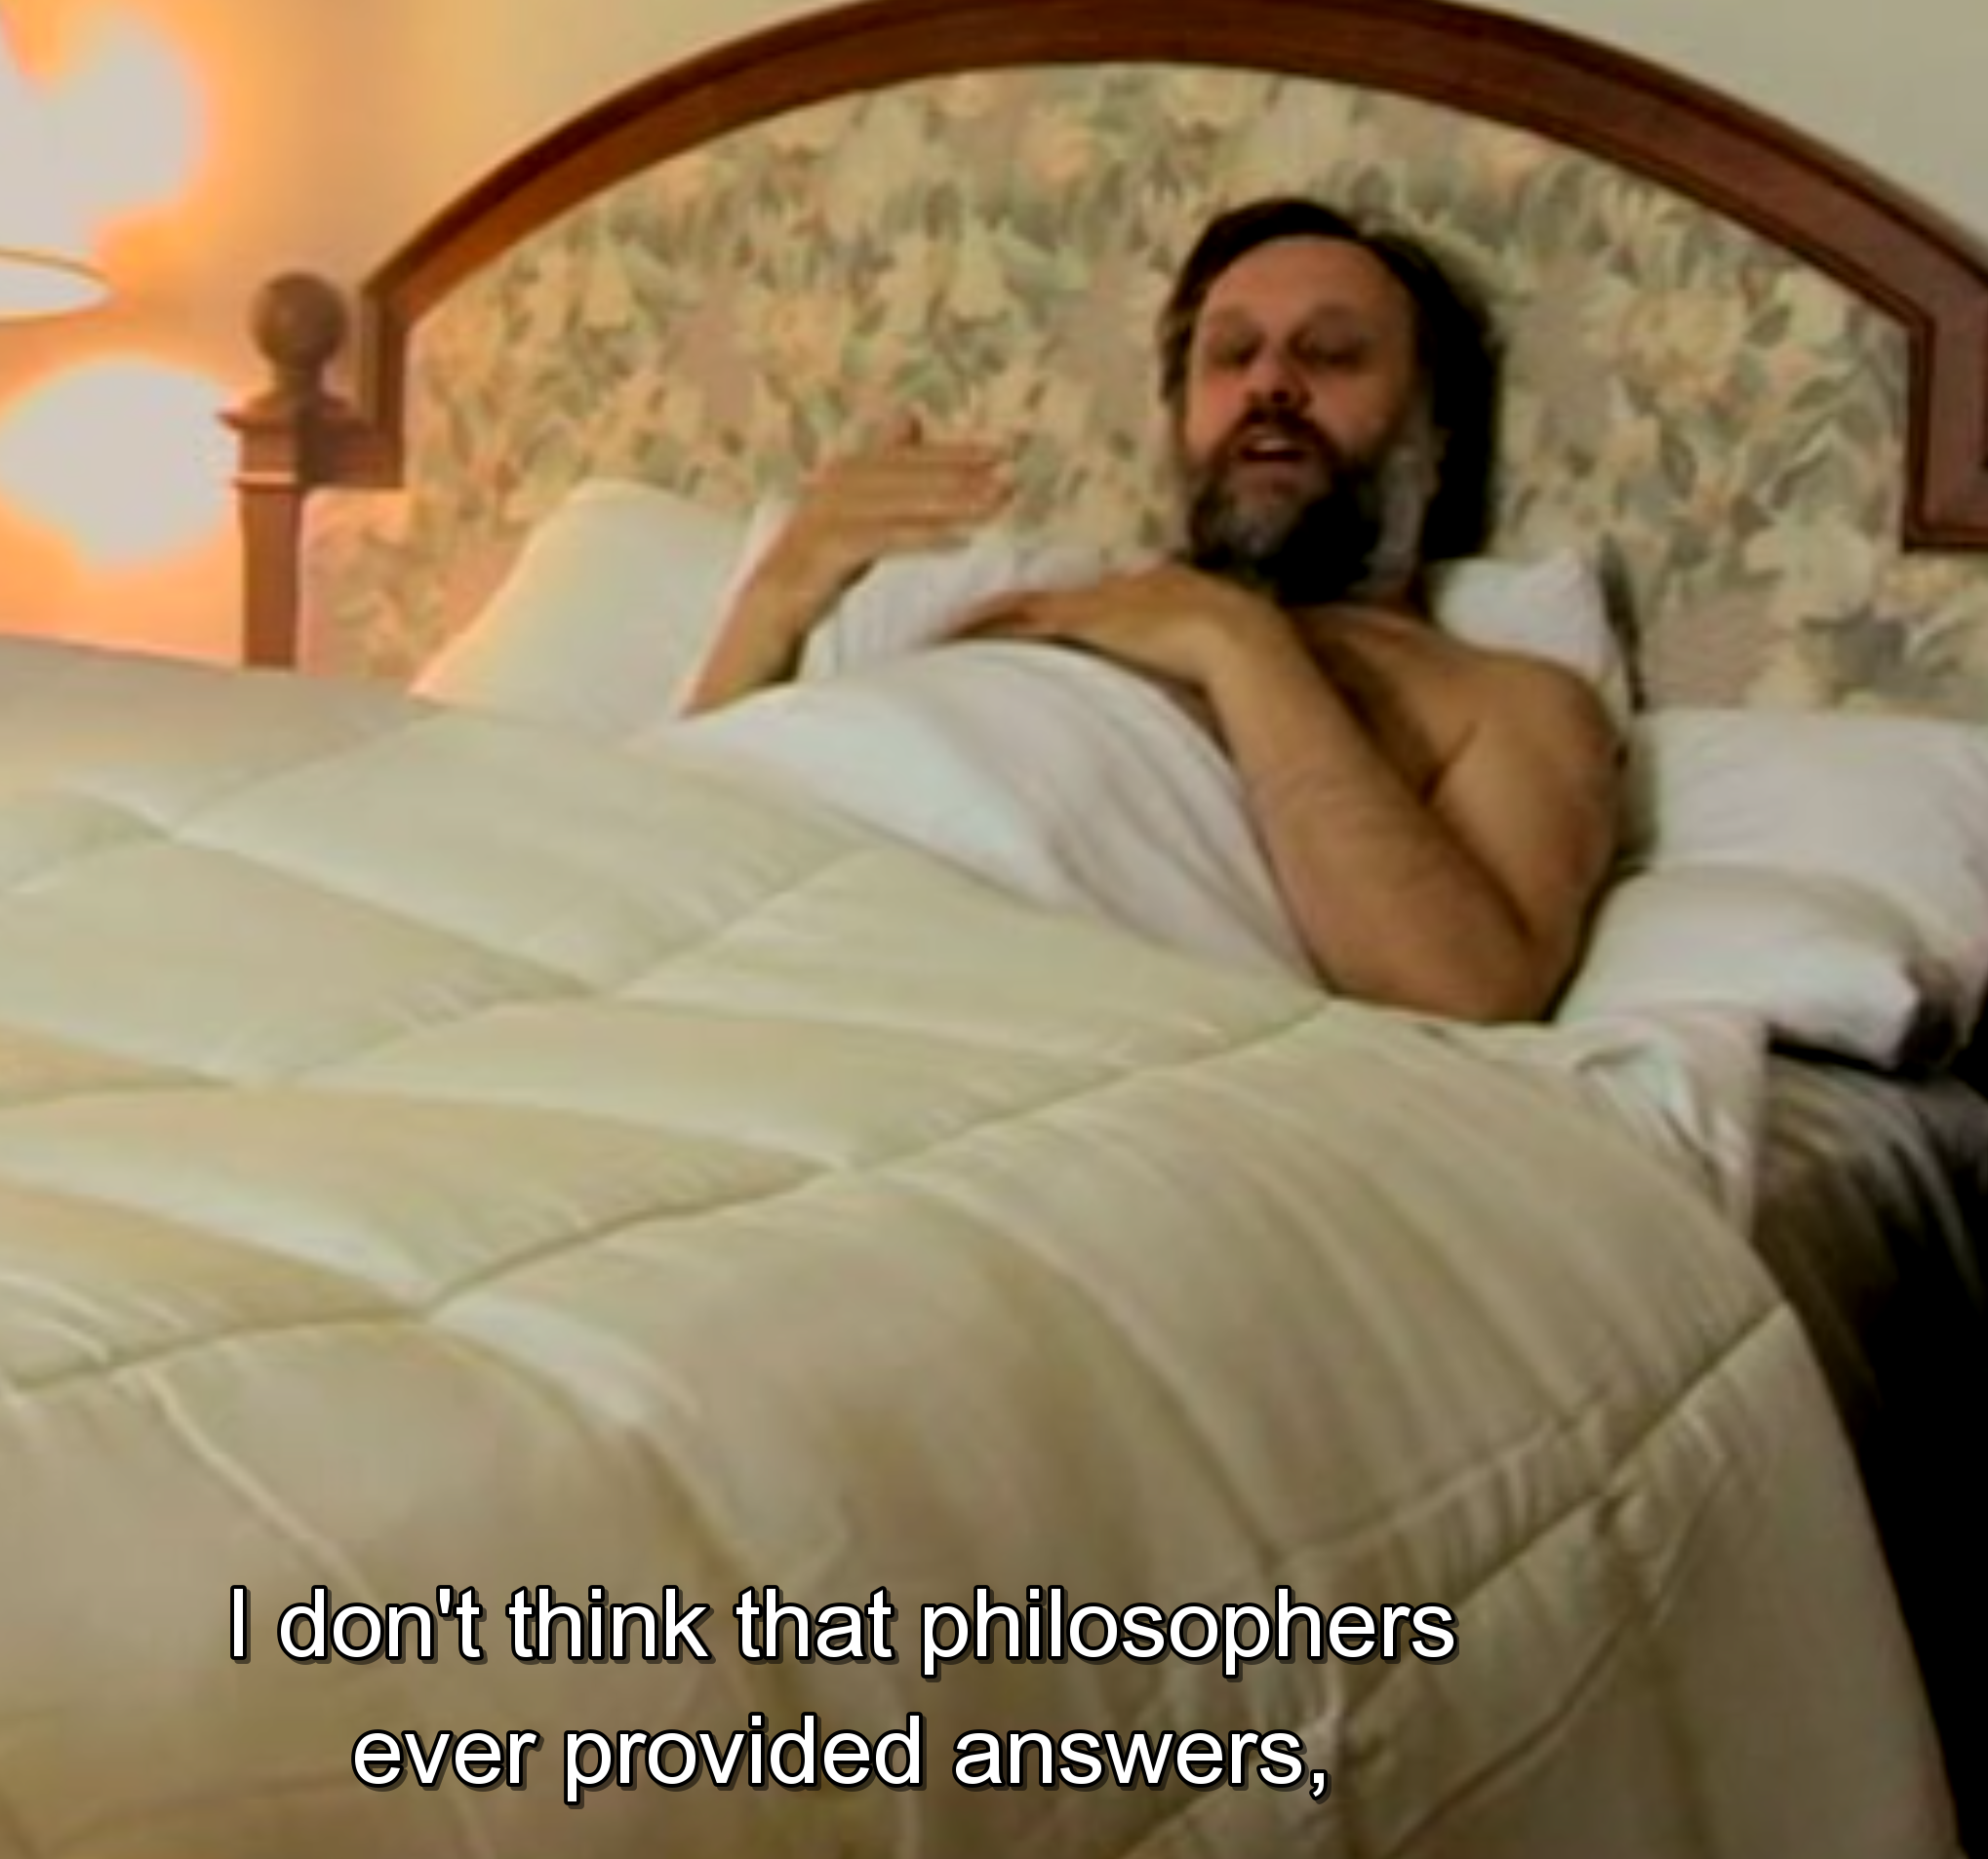
\includegraphics[width=0.5\textwidth]{images/template.png}
%	\caption{Template Bild}
%	\label{fig:template}
%\end{figure}

\end{document}
